\documentclass{article}

\usepackage{graphicx}
\usepackage{subcaption} % fig across two pages
\usepackage[margin=2cm,a4paper]{geometry}
\usepackage{lmodern}
\usepackage{tcolorbox}
\tcbuselibrary{listings,skins}
\usepackage{microtype}

% References - citations style of Nature
\usepackage[
backend=biber,
style=nature
]{biblatex}
% imported references: 
\addbibresource{all_references.bib}

\usepackage[colorlinks = true,
	linkcolor = blue,
	urlcolor  = blue,
	citecolor = blue,
	anchorcolor = blue
]{hyperref}
\urlstyle{same}
\usepackage[htt]{hyphenat}
\usepackage{placeins}
\usepackage{parskip}
\usepackage{xcolor}
	\definecolor{keyword}{HTML}{cc241d}
	\definecolor{string}{HTML}{98971a}
	\definecolor{comment}{HTML}{928374}


\usepackage{listings}
\usepackage{xcolor}

\definecolor{codegreen}{rgb}{0,0.6,0}
\definecolor{codegray}{rgb}{0.5,0.5,0.5}
\definecolor{codepurple}{rgb}{0.58,0,0.82}
\definecolor{backcolour}{rgb}{0.95,0.95,0.92}

\lstdefinestyle{mystyle}{
    backgroundcolor=\color{backcolour},   
    commentstyle=\color{codegreen},
    keywordstyle=\color{magenta},
    numberstyle=\tiny\color{codegray},
    stringstyle=\color{codepurple},
    basicstyle=\ttfamily\footnotesize,
    breakatwhitespace=false,         
    breaklines=true,                 
    captionpos=b,                    
    keepspaces=true,                 
    numbers=left,                    
    numbersep=5pt,                  
    showspaces=false,                
    showstringspaces=false,
    showtabs=false,                  
    tabsize=2
}

% Black version
\lstdefinestyle{nocolor}{
    keywordstyle=\color{black},
    commentstyle=\color{black},
    stringstyle=\color{black}
}

\lstset{%
language=bash,
style=mystyle,
breaklines=true,
showstringspaces=false,
frame=single} 

\begin{document}

\title{Building an Infrastructure as a Service on the Amazon Web Service Cloud}
\author{ilante}
% \date{\today}

\maketitle

\section{Creating an HTCondor Cluster for Training Support Vector Machines for Secondary Structure Prediction}

The aim of this project is to demonstrate how to build an Infrastructure as a Service (IaaS) on the \href{https://aws.amazon.com/}{Amazon Web Services} Platform. 
We chose \href{https://www.csie.ntu.edu.tw/~cjlin/libsvm/}{libsvm} \cite{chang_libsvm_2011}, 
a library for Support Vector Machines as application to run the test jobs, because training a model for classification is a computationally intensive task. 
In a real scenario it is necessary to perform a grid search, for finding the best hyperparameters for training the model \cite{gholami_chapter_2017}.
The IaaS we introduce in this project is an HTCondor cluster consisting of only three nodes; one \href{https://web.archive.org/web/20210531104015/https://www.independent.co.uk/life-style/gadgets-and-tech/news/github-master-slave-slavery-whitelist-language-inclusive-a9568576.html}{main} node and two worker nodes. 
The infrastructure can be expanded by simply replicating the worker node instance according to the needs of the application.
The main node was not set up as worker node to avoid the risk of overloading.
A shared storage that is directly attached to the main node is available to all worker nodes. This shared storage is implemented by the Network File System (NFS) protocol.
All scripts can be found in the projects \footnotesize \href{https://github.com/ilante/BDP-projcect-aws-main}{GitHub repository}.
%\cite{
%https://citeseerx.ist.psu.edu/viewdoc/summary?doi=10.1.1.14.473

\subsection{Initiating the Instances on the Amazon Web Services Cloud}
For this project we chose to use the cloud service provider Amazon Web Services (\href{https://aws.amazon.com/}{AWS}) as free credit was provided by the course, where we instantiated three Nodes: worker nodes and the main node were all run on CentOS Linux 8.
%#############################################################################################
For the main node, we chose the \texttt{t2.micro} instance type with a 10 Gb SSD as root storage.
% \begin{lstlisting}[language=bash]
% centos@main:~$ df -h
% Filesystem      Size  Used Avail Use% Mounted on
% devtmpfs        374M     0  374M   0% /dev
% tmpfs           403M     0  403M   0% /dev/shm
% tmpfs           403M   11M  393M   3% /run
% tmpfs           403M     0  403M   0% /sys/fs/cgroup
% /dev/xvda1       10G  3.4G  6.7G  34% /
% /dev/xvdf1       30G  120M   28G   1% /data
% tmpfs            81M     0   81M   0% /run/user/1000
% \end{lstlisting}
For the worker nodes, we chose the \texttt{t2.small} instance type with a 16 Gb SSD as root storage.
\begin{figure}[!h]
    % \center%
    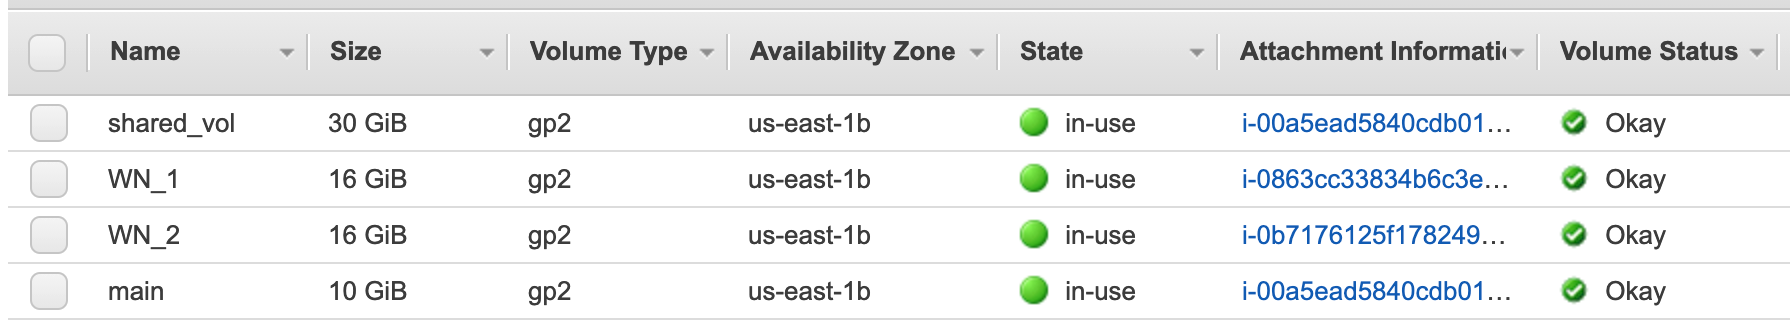
\includegraphics[width=0.7\textwidth]{./img/root_storage_shared_vol.png}
\end{figure}
% Maybe use text instead of screenshot?
% \begin{lstlisting}
% centos@ wn_1 :~$ df -h
% Filesystem          Size  Used Avail Use% Mounted on
% devtmpfs            878M     0  878M   0% /dev
% tmpfs               907M     0  907M   0% /dev/shm
% tmpfs               907M   17M  891M   2% /run
% tmpfs               907M     0  907M   0% /sys/fs/cgroup
% /dev/xvda1           16G  3.0G   14G  19% /
% 172.31.1.180:/data   30G  120M   28G   1% /data
% tmpfs               182M     0  182M   0% /run/user/1000
% \end{lstlisting}

% %#############################################################################################
To ensure that the machines are able to communicate through private IPv4 addresses, all nodes were instantiated in the same availability zone (\texttt{us-east-1b}) and the same security group. 
The security group is set to allow Secure Shell Protocol (\textit{SSH}) connection, port 22, from everywhere, provided the user has the matching key.
We did not open it exclusively to our local public IP, because throughout the project we are accessing the internet from different geographic locations. 
The IP address of my private laptop will change whenever I'm accessing from a different WiFi network, but also when the router is restarted. 
All Transmission Control Protocol (\textit{TCP}), was allowed for machines of the \textit{same} security group, thus allowing for file transfer \cite{cerf_protocol_1974}. 
Further, HTCondor deamons use a dynamically assigned port. 
All ICMP was allowed between machines sharing the same security group, to enable \textit{ping} e.g. for checking if a certain host is online and other testing purposes.
\begin{figure}[!h]
    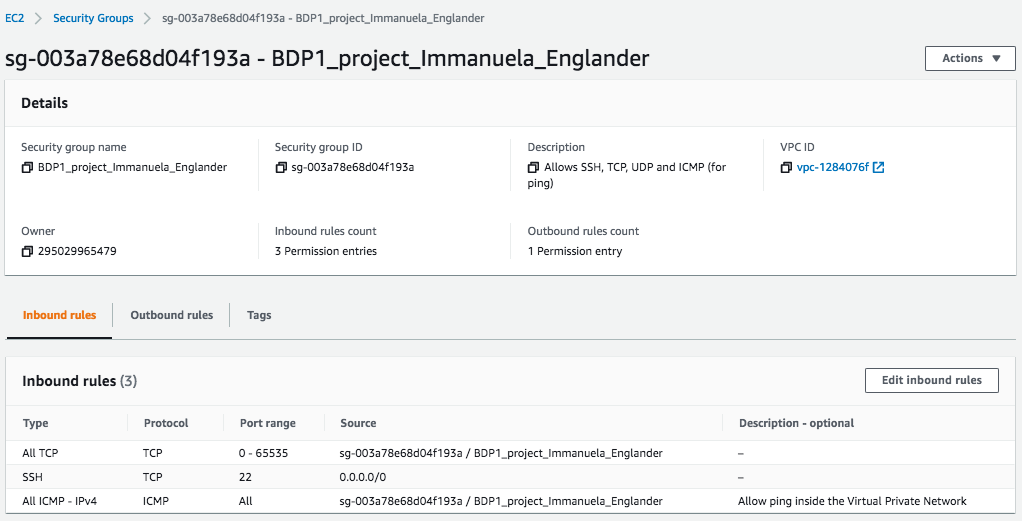
\includegraphics[width=0.75\textwidth]{./img/security_groups.png}
\end{figure}
\newpage
\subsection{Configuring the Main Node}
We changed the PS1 prompt of the main node ensuring any user logging in, can recognize it right away.
This was done for reducing the risk of modifying any configuration on the wrong machine.

\begin{figure}[!h]
    % \center%
    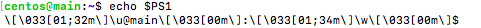
\includegraphics[width=0.58\textwidth]{./img/prompt.png}
\end{figure}
\FloatBarrier%

First, we installed dependencies for HTCondor \cite{condor-practice} on both main and worker nodes with the commands shown below:

\begin{lstlisting}[language=bash]
sudo su -
# SELinux policies for container runtimes, dependency for HTcondor
wget mirror.centos.org/centos/7/extras/x86_64/Packages/container-selinux-2.107-3.el7.noarch.rpm 

yum localinstall container-selinux-2.107-3.el7.noarch.rpm 

yum clean all 
\end{lstlisting}

Then we created a new yum repo for HTCondor and copied the stable HTcondor into the new repo:
\begin{lstlisting}[language=bash]
# creating new yum HTcondor repo
wget http://research.cs.wisc.edu/htcondor/yum/repo.d/htcondor-stable-rhel7.repo 
#copy to my new yum repo
cp htcondor-stable-rhel7.repo /etc/yum.repos.d/ 
\end{lstlisting}

First we obtained the key used for authentication of the repo, and told the system to trust the key. Thereafter we installed all packages of HTCondor as follows:
\begin{lstlisting}[language=bash]
# obtain key
wget http://htcondor.org/yum/RPM-GPG-KEY-HTCondor
# import and trust
rpm --import RPM-GPG-KEY-HTCondor
# install HTCondor
yum install condor-all 
\end{lstlisting}

Then we enabled and started HTCondor with the following commands:
\begin{lstlisting}[language=bash]
systemctl enable condor
systemctl start condor
\end{lstlisting}

To ensure that the installation was successful, we checked the status of the software we used the command showing in the screenshot on the next page:

\begin{figure}[!h]
    \center%
    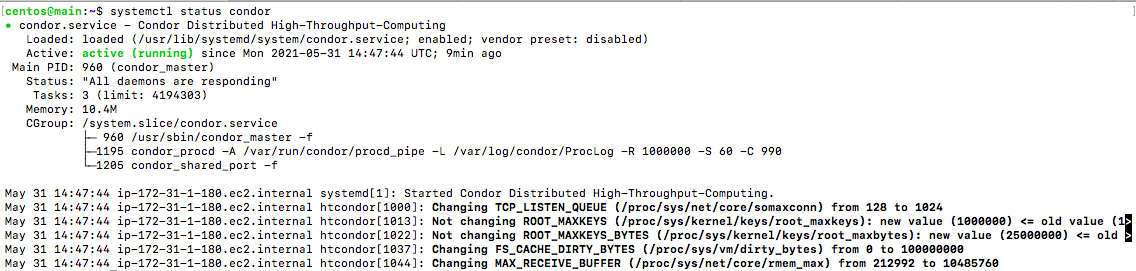
\includegraphics[width=\textwidth]{./img/condor_status.png}
\end{figure}

For basic configuration, we appended the following lines to the main nodes HTCondor configuration file, found in the path:\\
\texttt{/etc/condor/condor\_config}:

\begin{lstlisting}[language=bash]
# Main Node IP
CONDOR_HOST = <Main_Node_private_IP>

# Main Node config 
DAEMON_LIST = COLLECTOR, MASTER, NEGOTIATOR, SCHEDD

HOSTALLOW_READ = *
HOSTALLOW_WRITE = *
HOSTALLOW_ADMINISTRATOR = *
\end{lstlisting}

To make sure that the changed settings take effect, we restarted HTCondor and checked the status again with the following command:
\begin{lstlisting}
sudo systemctl restartcondor
condor_status
\end{lstlisting}

\subsection{Setting up Network File System on the MASTER Node}

To set up a Network File System (NFS) we first had to create a new disk ("Volume" in AWS lingo).
From the Amazon Elastic Compute Cloud (EC2) side bar menu under 'Elastic Block Storage' we selected 'Volumes' and picked the default EBS General Purpose SSD (gp2) with 30 GiB capacity and attached it to the main node. 
This was done by checking the volume and subsquently opening the 'Actions' dropdown and selecting 'Attach Volume'.

Then via the console we added the new volume to the partition list via the \texttt{fdisk} utility: \newline
\texttt{fdisk /dev/$<$my\_new\_volume$>$} was added to the partition table using the default parameters. The changes where saved using the \texttt{w} (write) command. Then we created the file system on the partition we just created by issuing the following command: 

\begin{lstlisting}
# Formatting my new partition
mkfs.ext4 /dev/<my_partition>
\end{lstlisting}

By modifying the \texttt{/etc/fstab} file (see snippet below) we ensured the main node will mount the volume automatically upon boot onto the directory \texttt{/data}
\begin{lstlisting}
/dev/<my_newly_formatted_partition>              /data    ext4   defaults                0 0
\end{lstlisting}

I installed the NFS by issuing the commands below:
\begin{lstlisting}[language=bash]
yum install nfs-utils rpcbind
systemctl enable nfs-server
systemctl enable rpcbind     # starts the service upon boot
systemctl start rpcbind
systemctl start nfs-server
# checking if install, enable start worked fine
systemctl status nfs-server 
\end{lstlisting}

We created a new directory in \texttt{/data} which was then used as mount point for the shared FS. 
We appended the following line to the NFS configuration file in \texttt{/etc/exports} to expose \texttt{/data} to all the machines in my virtual private network, or virtual private cloud (VPC) in AWS lingo.
This allows any computer in the VPC to connect to the NFS server and access the shared FS.
This poses little security risk as only we can create new machines belonging to the same VPC, and it is a secure solution as long as only HTCondor Main and worker nodes are hosted in this VPC. 
If I, as admin wanted to launch any other application we would have to host it on a different VPC.
\begin{lstlisting}
/data 172.31.0.0/16(rw,sync,no_wdelay)
\end{lstlisting}
%#########################################################################################################
%#########################################################################################################
The range of IP's of my virtual private network can be found by checking one of the instances and clicking onto the VPC link marked in pink (see screenshots below). From there you can find the IP range in the column "IPv4 CIDR" marked in pink.
\begin{figure}[!h]
    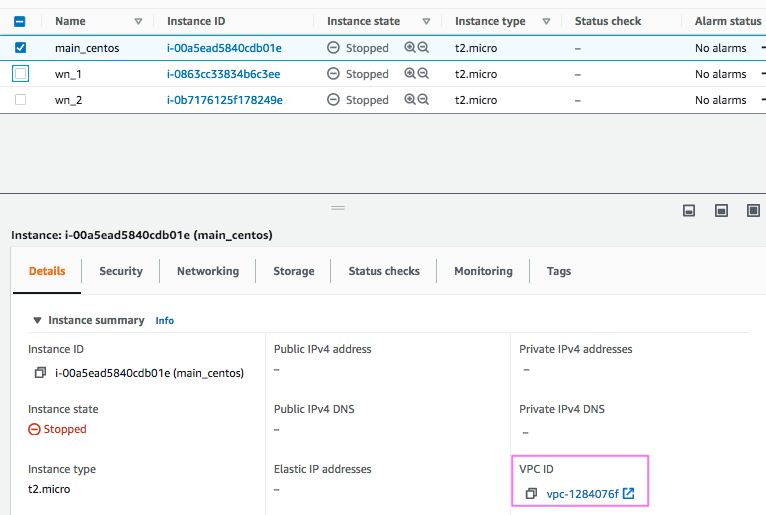
\includegraphics[width=0.82\textwidth]{./img/find_vpc.png}
\end{figure}

%#########################################################################################################
%#########################################################################################################
\begin{figure}[!h]
    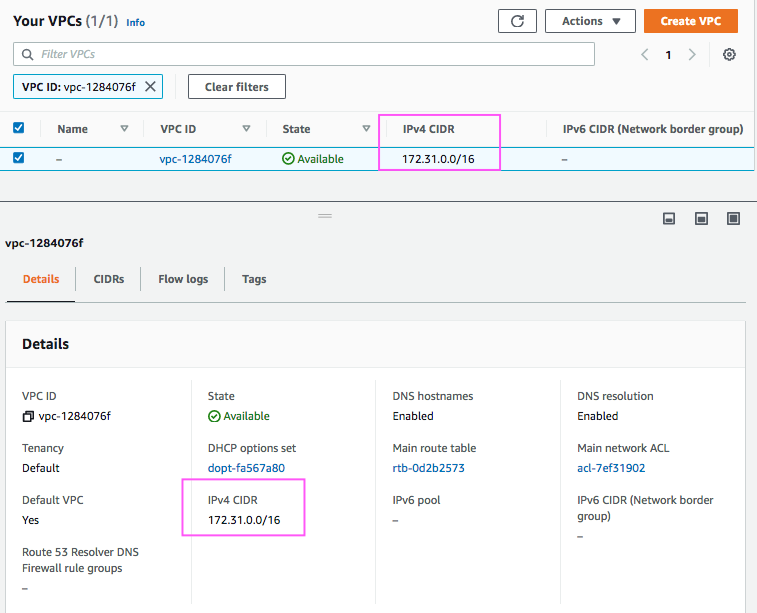
\includegraphics[width=0.82\textwidth]{./img/ip_range.png}
\end{figure}

I changed the rights to the shared directory to grant read, write and execute access for all users.
\begin{lstlisting}[language=bash]
sudo chmod 777 /data
\end{lstlisting}

\subsection{Configuring the Worker Node}
For configuring the worker node we first instantiated a \texttt{t2.micro} machine with CentOS Linux 8\@. Again, for better orientation, we changed the prompt to:
\begin{figure}[!h]
    % \center%
    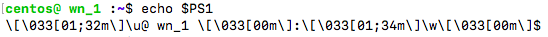
\includegraphics[width=0.65\textwidth]{./img/prompt_wn.png}
\end{figure}
\FloatBarrier%

For the installation of HTCondor on this worker node the same procedure was followed as described in section 1.2.
The \texttt{/etc/condor/condor\_config} file however, had to be configured differently for the worker node by appending the following lines to it:
\begin{lstlisting}
# Main Node IP
CONDOR_HOST = <Main_Node_private_IP>

# Worker Node config
DAEMON_LIST = MASTER, STARTD

HOSTALLOW_READ = *
HOSTALLOW_WRITE = *
HOSTALLOW_ADMINISTRATOR = *
\end{lstlisting}

To be able to mount the shared volume on the worker node the NFS client library was installed issuing the commands below:
\begin{lstlisting}[language=bash]
yum install nfs-utils
\end{lstlisting}

To ensure \texttt{/data} was mounted upon boot the following line was added to the worker nodes \texttt{/etc/fstab}:
\begin{lstlisting}
<private_IP_of_MAIN_node>:/data      /data    nfs    defaults                0 0
\end{lstlisting}
And then we mounted it with:
\begin{lstlisting}
mount -a
\end{lstlisting}

Even though the commands were successful, we ran \texttt{ll /data} from the worker node. We also created a file from the worker to verify that the permissions were set correctly.
Then we installed the \texttt{libsvm} application on the worker node via \cite{chang_libsvm_2011}:
\begin{lstlisting}[language=bash]
sudo yum install libsvm
\end{lstlisting}

\section{Installing Docker on Main and Worker Nodes and Creating an Image on my Local Machine}
Docker is an open-source software project that is used for packing and shipping applications in containers and automating the deployment thereof \cite{merkel2014docker, noauthor_docker_nodate}.
First we created a Dockerfile to create an image on my local machine:
\lstinputlisting[language=bash]{scripts/Dockerfile}
We built and tagged the image which can also be found online on \href{https://hub.docker.com/r/ilante/centos8_libsvm}{Docker Hub} \cite{noauthor_docker_nodate}:
\lstinputlisting[language=bash]{scripts/stdout_docker_tag_image.log}
Lastly we pushed the image to Docker Hub such that the worker in my IaaS can later pull it.
\lstinputlisting[language=bash]{scripts/stdout_docker_push_image.log}

From the worker node we ensured functionality by issuing both the \texttt{svm-predict} and the \texttt{svm-train} commands, as shown in the following snipped copied and pasted from the terminal:
\lstinputlisting[style=nocolor]{scripts/stdout_docker_image_test.log}
\newpage
\subsection{Configuring Condor to use Docker}
To allow HTCondor to run Dockerized jobs we changed the configuration of the worker nodes by adding the condor user to the Docker group:
\begin{lstlisting}
sudo usermod -aG docker condor
\end{lstlisting}
Thereafter we updated the condor configuration on the worker nodes to allow the shared volume to be mounted on the containers by appending the following lines to \texttt{/etc/condor/condor\_config}:
\begin{lstlisting}
##--------------------------------------------------------------------
## Docker Volume Config
##--------------------------------------------------------------------
# Defining only one docker volume
DOCKER_VOLUMES = SHARED_DATA
# Assigning the /data directory to docker volume
DOCKER_VOLUME_DIR_SHARED_DATA = /data
# Mount SHARED_DATA volume in all containers handled by HTcondor
DOCKER_MOUNT_VOLUMES = SHARED_DATA
\end{lstlisting}

To update the status of the cluster we ran a command for concluding the reconfiguration.
\begin{figure}[!h]
    
\includegraphics[width=0.55\textwidth]{img/condor_reconfig.png}
\end{figure}
\FloatBarrier

For veryfying that the reconfiguration was successful  we checked the cluster for Docker enabled nodes:
\begin{figure}[!h]
    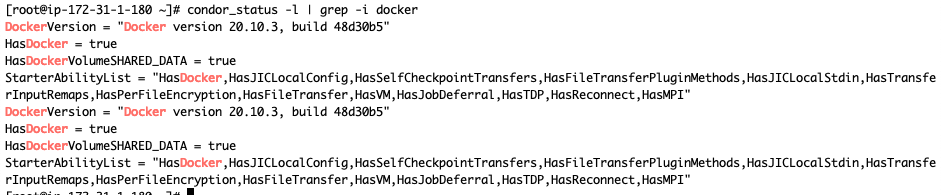
\includegraphics[width=\textwidth]{img/condor_status_grep_i_docker.png}
\end{figure}



%EXPANDING cluster via snapshot
\subsection{Expanding the Cluster}
Given that workers are stateless, while the master is stateful, the number of workers can be changed without taking the cluster offline.
To be able to expand my cluster with minimal effort we created an image of my fully configured worker node.
From this image the administrators of the cluster can scale the cluster horizontally according to their needs (and financial resources).
For the scope of this project we contented myself with second worker node that did not require any manual configuration, created from the image you can see below.
\begin{figure}[!h]
    \center%
    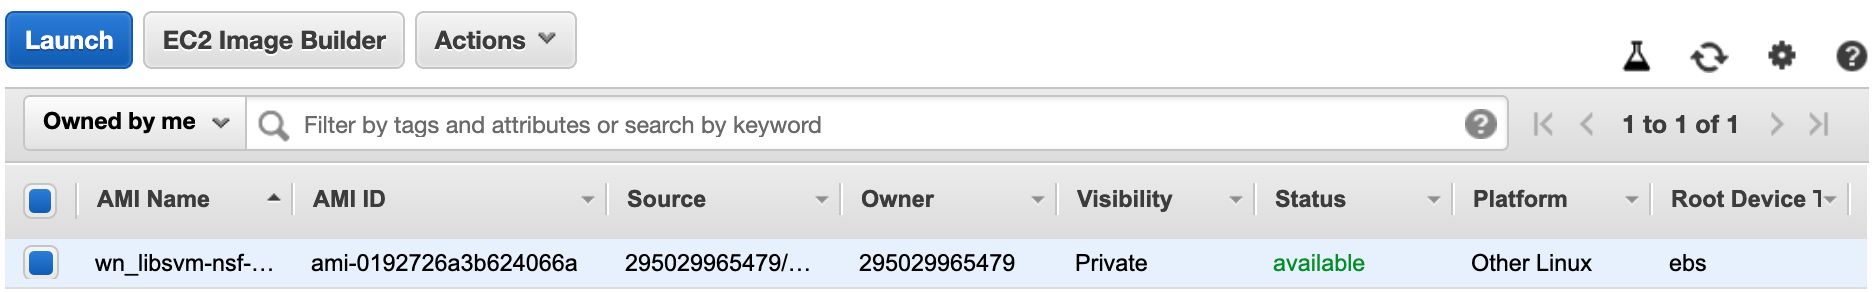
\includegraphics[width=\textwidth]{img/wn_image.png}
\end{figure}

\section{Submitting an Support Vector Machine Test Job to my HTCondor Cluster}
Support Vector Machines (SVM) are a supervised machine learning algorithm first published as \textit{Support Vector Networks} by Corinna Cortes and Vladimir Vapnik in 1995 \cite{cortes_support-vector_1995}. The library that was implemented in this project  is called \href{https://www.csie.ntu.edu.tw/~cjlin/libsvm/}{\texttt{libsvm}} \cite{chang_libsvm_2011}.
The SVM algorithm achieves classification by finding the optimal hyperplane that separates two classes while maximizing the \textit{margin} defined as the distance between the support vectors \cite{gholami_chapter_2017}.
The maximum margin hyperpalne is used as a decision boundary for classifying new data points.
Inspired by the extremely long training times of SVM used during another project we decided to choose this application. 
For this algorithm it is paramount to find the best values for the hyperparameters $C$ and $\gamma$ by performing a grid search.
The use case of the grid search shall be explored for a use case when predicting the expected costs. % EXPECTED costs

\subsection{Choosing Input Executable and Job Files} %for the Minimal \texttt{libsvm} Job
For the scope of this project we chose six input files of increasing size to train a SVM model which was subsequently used to predict protein secondary structure from a single testing file.
These files where generated in a previous \href{https://github.com/ilante/LB-2-project-GOR-vs-SVM}{project} in the following fashion:
The \texttt{libsvm} programs (predict and train) take input data in the format of numerical vectors for both training and prediction. 
Thus we used a \href{https://github.com/ilante/LB-2-project-GOR-vs-SVM/blob/master/scripts/generate_svm_input.sh}{script} that transforms the data from a profile windows, into a 20 (amino acids) by 17 (window size) vector. These 340 feature vectors were subsequently matched to the class of the central residue Helix, Strand or Coil (H, E or C). 
The secondary structure was then encoded as 1 for H, 2 for E and 3 for C. 
% As we were dealing with three-class classification the one versus all others approach was implemented such that prediction is performed comparing the values of the three binary discrimination functions.
No additional larger testing files for prediction were used, because bulk time of the application is spent on testing, while in a real use case the file to be predicted would not have a significant influence. % XXXXX imporve style

The test job consisted in training six SVM models from the files numbered $0 - 5$ shown below with the \texttt{svm-train} function of \texttt{libsvm}.
Each of the six models was subsequently used to predict the same input file \texttt{test\_data.svm}.
The sizes of the minimal input files were as follows: 
% \newpage
% [language=bash]
\begin{lstlisting} 
centos@main:~/BDP-projcect-aws-main/in_train_tiny$ ll -h *.svm
-rw-rw-r--. 1 centos centos  16M Jun 17 20:52 test_data.svm
-rw-rw-r--. 1 centos centos 5.1M Jun 16 16:44 train0.svm
-rw-rw-r--. 1 centos centos  11M Jun 16 16:47 train1.svm
-rw-rw-r--. 1 centos centos  16M Jun 16 16:50 train2.svm
-rw-rw-r--. 1 centos centos  21M Jun 16 16:52 train3.svm
-rw-rw-r--. 1 centos centos  26M Jun 16 16:53 train4.svm
-rw-rw-r--. 1 centos centos  31M Jun 16 16:54 train5.svm
\end{lstlisting}
% #########################################################################################################
% #########################################################################################################
% \subsubsection{Preparing Executable and Job File for HTCondor}
The simple \texttt{bash} script that serves as the executable for condor is shown below:
\lstinputlisting[language=bash]{scripts/svm_test_predict_exec.sh}
% In the following listing you can see t
The job file (\texttt{svm\_test\_predict.job}) for HTCondor was set to request 1024 MB which is identical to the memory (\texttt{-m 1024}) requested in line 15 of the \texttt{svm\_test\_predict.job} file (above). We requested 1 CPU, as \texttt{libsvm} is not a multi-threaded application which means We cannot take advantage of more than one CPU.
\lstinputlisting[language=bash]{./scripts/svm_test_predict.job}

I ran six instances of the test job on the cluster. Given the settings described previously, the jobs ran in pairs, one on each worker node (see screenshot below).
% The following outputs of \texttt{condor\_q} and \texttt{condor\_status} were recorded after submission:

\begin{figure}[!h]
    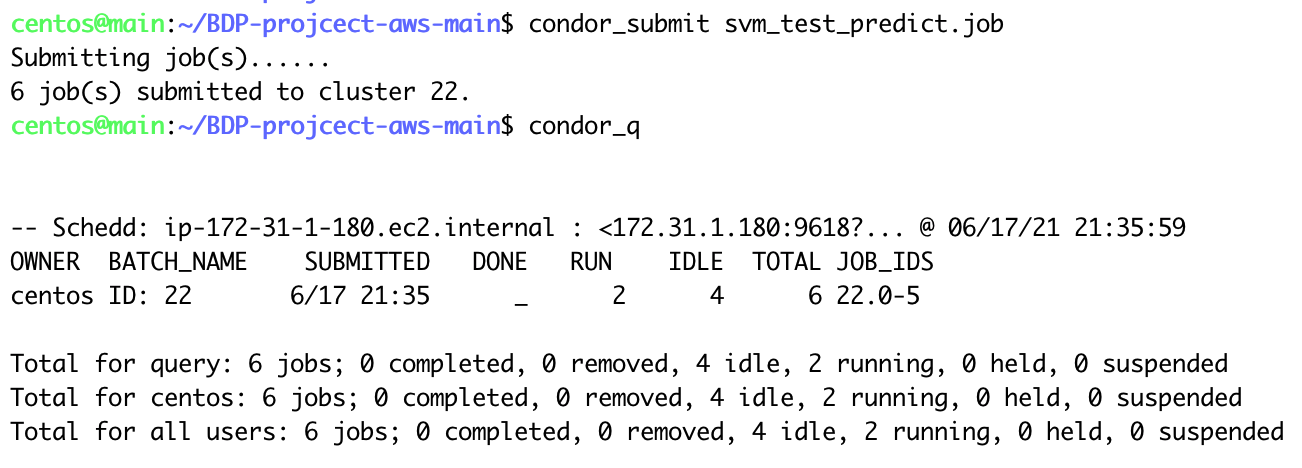
\includegraphics[width=0.7\textwidth]{./img/condor_submit_q}
\end{figure}
\FloatBarrier%

The cluster completed the task successfully producing 6 SVM models and 6 predictions: % six or 6?
\begin{figure}[!h]
    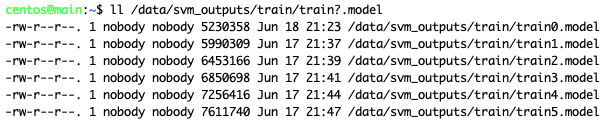
\includegraphics[width=0.7\textwidth]{./img/condor_output.model.png}
\end{figure}
\FloatBarrier%

The duration of each task ranged from 100 to 383 seconds, with an average of 227.7 seconds.

\begin{figure}[!h]
    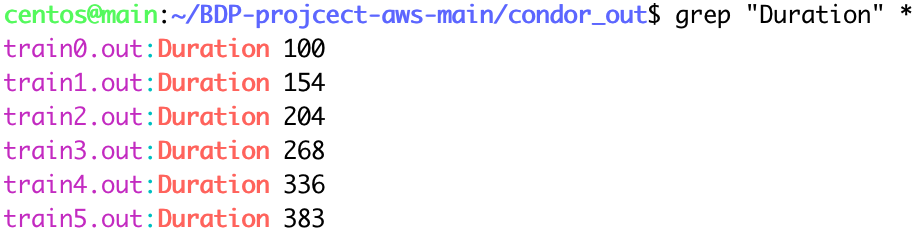
\includegraphics[width=0.65\textwidth]{./img/condor_duration_job.png}
\end{figure}
\FloatBarrier%

\section{Running an Identical Job in Docker Containers}
To run an identical job in Docker Containers, we modified the job file for HTCondor, 
in order to ensure that none of the previously generated data would be overwritten. 
This was done in part by creating a new output directory reserved for the Docker job output (logs, errors and output).
Note that the universe (line 60) has to be set to docker.
As the model was saved in the shared volume, here the name of the output was changed to make it distinguishable from the other models:
\lstinputlisting[language=bash]{scripts/svm_test_predict_docker.job}
Each of the job instances ran successfully.
The duration of each of the six job was slightly longer than in the non-containerized version (see section 2.2); ranging from 105 to 397 seconds. 
Given that the cluster is composed of virtual machines, running Docker adds another layer of abstraction and isolation which may have led to this small performance loss.

Depending on the needs of the job Docker can provide higher flexibility and reproducibility in case of highly costumized binaries.
As previously mentioned, by the time of writing, \texttt{libsvm} does not provide a multi-threaded implementation for any major linux distribution.
Chang and Lin do how ever provide
% \href{https://www.csie.ntu.edu.tw/~cjlin/libsvm/faq.html#f432}{} for some reason the "#" turns into "%" when clicking the link
\href{http://gourl.gr/c4hm}{instructions} on how to compile such version in house \cite{chang_libsvm_2011}.
Such implementation may then be put into a container and deployed to the cluster for convenience of its users.
Using this hypothetical multi-threaded implementation of \texttt{libsvm} could greatly reduce the time for training the models.

% https://www.csie.ntu.edu.tw/~cjlin/libsvm/faq.html#f432
% While software usually runs faster in Docker than the same software running on a virtual machine,
% however, in our case, the same software is run once on several virtual machines forming a cluster.
% And in the second run the software is run on that cluster of virtual machines.
% we attribute the increased time to the fact that to Docker provides one more layer of abstraction and isolation.
% \begin{figure}[!h]
%     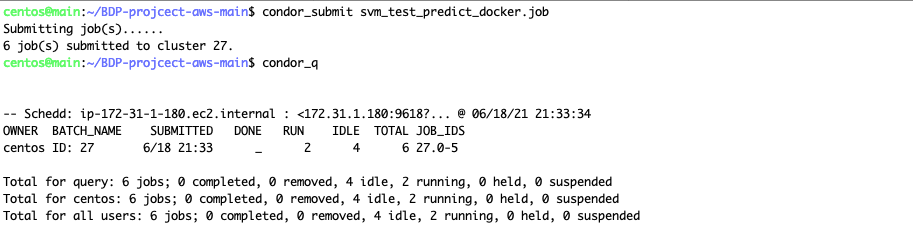
\includegraphics[width=\textwidth]{./img/condor_submit_q_docker.png}
% \end{figure}
% \FloatBarrier%

\begin{figure}[!h]
    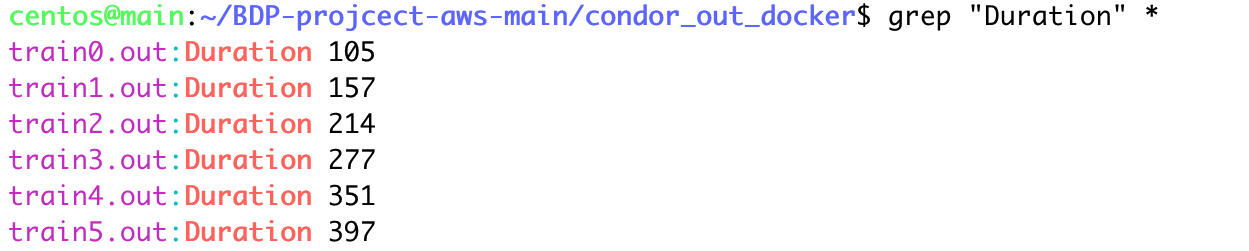
\includegraphics[width=0.75\textwidth]{./img/condor_duration_job_docker.png}
\end{figure}
\FloatBarrier%

\subsection{Data Management Model}
The data model is based on the following assumptions: The input data is sensitive data and therefore cannot be shared with other users of the infrastructure.
The logs, outputs and errors are not shared for the scope of not polluting the shared volume with this kind of volatile date.
The models produced by the training, however, cannot be traced back to the sensitive input, and are to be shared with the other users for classification purposes.
Given these assumptions and the infrastructure, described in section 1, the data model is the following:
The executable, the input files for training the model and the test file for validating the model \texttt{test\_data.svm} are passed via the sand box. 
This choice is justified by the size of the data and the number of jobs.
Each of the generated models are saved to the shared volume as they must be available to other users.
The standard output, condor log and condor error files are retrieved via the output sandbox to be available to the job submitter for inspection and debugging reasons.

\section{Evaluating the Execution Time}
As previously mentioned, the input chosen was of increasing size. From this data the RAM utilization and execution time by input size was plotted using several python libraries (\href{https://github.com/ilante/BDP-projcect-aws-main/blob/main/stats/HTcondor_stats.ipynb}{GitHub}). 
The plots show that the jobs scale linearly which is congruent with the findings of Bottou et al. who found that running an SVM, space and time complexity are linear with respect to the number of support vectors \cite{Bottou2007SupportVM}.
\begin{figure}[h]

\begin{subfigure}{0.5\textwidth}
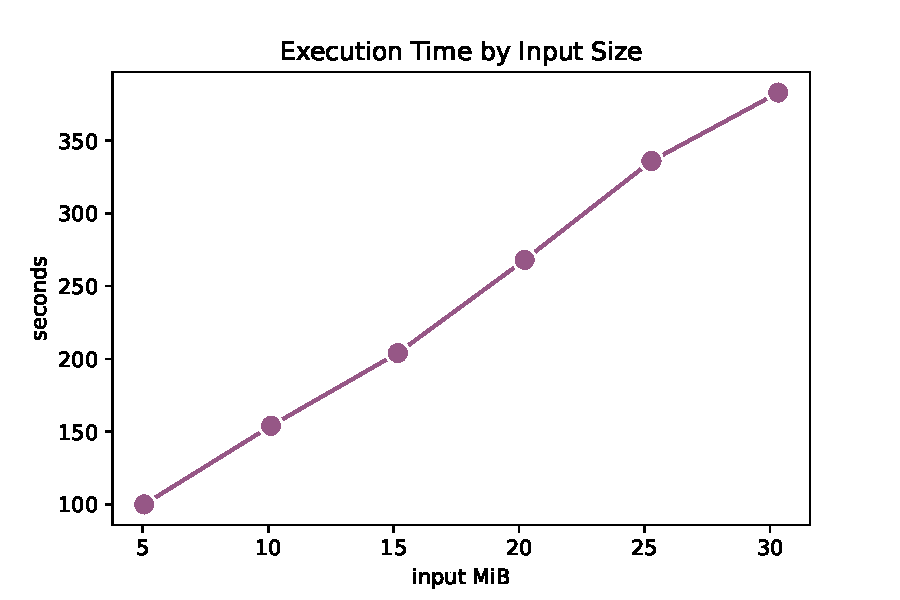
\includegraphics[width=0.9\linewidth]{img/stats/execution_by_input_size.pdf} %, height=6cm
% \caption{Caption1}
\label{fig:subtime1}
\end{subfigure}
\begin{subfigure}{0.5\textwidth}
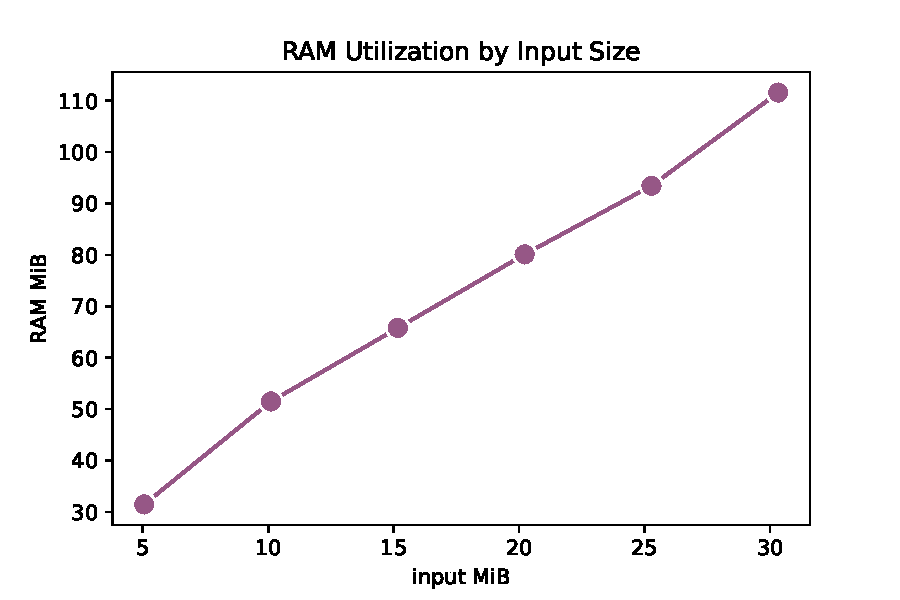
\includegraphics[width=0.9\linewidth]{img/stats/ram_utilization_jobs.pdf} %, height=6cm
% \caption{Caption 2}
\label{fig:subram2}
\end{subfigure}

\caption{Time (left) and RAM (right) used for each of the six input files}
\label{fig:image2}
\end{figure}
% \FloatBarrier
\begin{figure}[h]

\begin{subfigure}{0.5\textwidth}
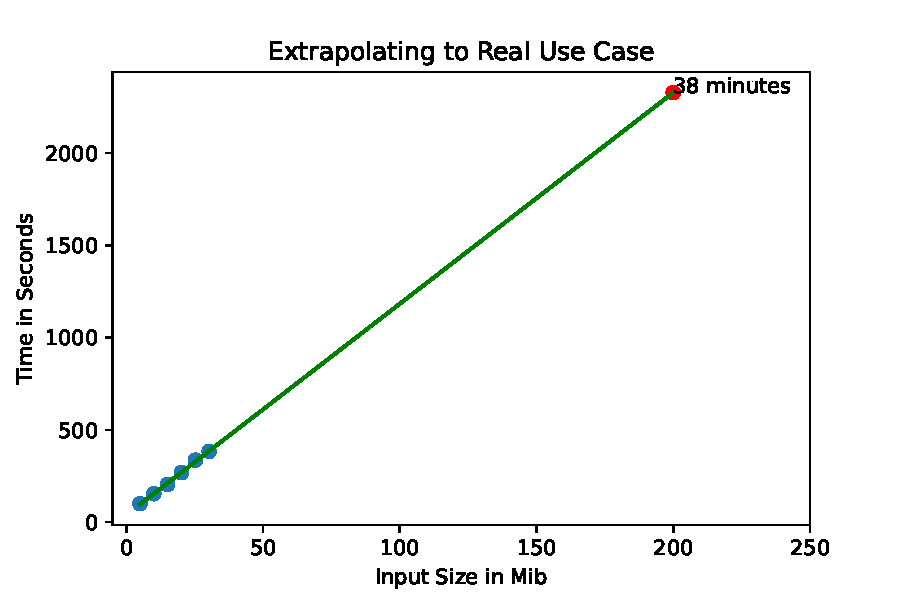
\includegraphics[width=0.9\linewidth]{img/stats/extrapolating_time_label.pdf} %, height=6cm
% \caption{Caption1}
\label{fig:subextra1}
\end{subfigure}
\begin{subfigure}{0.5\textwidth}
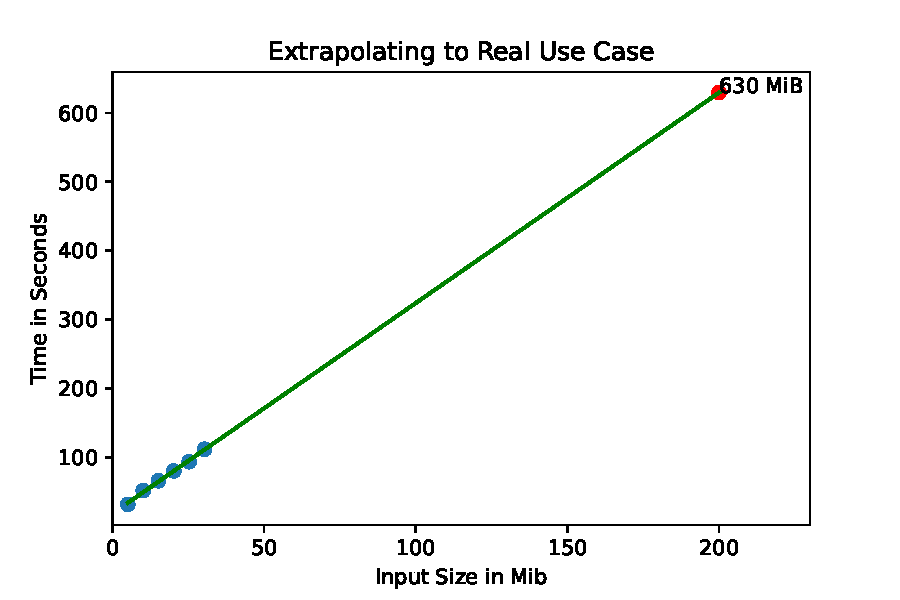
\includegraphics[width=0.9\linewidth]{img/stats/extrapolating_ram.pdf} %, height=6cm
% \caption{Caption 2}
\label{fig:subextra2}
\end{subfigure}

\caption{In a real use case with a training input of 200 MiB the expected runtime is 38 minues and the expected RAM usage is 630 MiB}
\label{fig:image3}
\end{figure}
\FloatBarrier

\subsection{Extrapolating to a Realistic use case}
Training a model with an input file of 200 MiB, which would correspond to roughly 1200 sequences.
This number was chosen, based on the number of sequences selected by the developers of JPred4, a protein secondary structure prediction server, as it is critical to have training data that are representative of the protein space in order to be able to generate a model that is capable of generalizing to unseen data.  \cite{drozdetskiy_jpred4_2015-1}.

\subsection{Expected Costs of a Non-Trivial Application} % for a Realistic Grid Search}
The execution of a grid search for determining the best hyperparameters is a plausible non-trivial use case that could be addressed by this HTCondor cluster that we have developed.
To execute an effective grid search entails to train SVM models using 10 combinations of the hyperparameters $C$ and $\gamma$.
For each of the combinations a five-fold cross validation should be carried out based splitting the training set that holds 1200 sequences.
This approach would require the training 50 different models.

One of the advantages of the IaaS is that horizontal up-scaling can be done easily as described in section 2.2.
This would allow us to replicate the worker nodes to achieve a cluster of 25 worker nodes with 2 vCPUs per node. 
Each of the workers would run 2 jobs in parallel amounting to an up-time of 38 minutes for running the entire task of training 50 models.

These 25 worker nodes would be orchestrated by a main node of the same make and size, thus the cluster would be comprised of 26 identical nodes.
This hypothetical set up of such a large number of small nodes is preferred over just two large worker nodes given that the \href{https://aws.amazon.com/ec2/pricing/on-demand/}{AWS pricing} 
shows that machines endowed with high numbers of cores are significantly more expensive than many small machines amounting to the same number of cores (see figure below) \cite{noauthor_ec2_nodate}.
Further, in case of job failure, we can take advantage of the pay-per-use model in the AWS cloud: The number of nodes needed to complete the task would stay up and running, while nodes that have produced a model successfully may be shut down and not payed for.

The proposed set-up of 26 t4g.medium nodes would require merely \$ 0.553 for completing the task in 38 minutes, provided it ran successfully on the first attempt.
The calculation of the of the expected cost is outlined in the \href{https://github.com/ilante/BDP-projcect-aws-main/blob/main/stats/HTcondor_stats.ipynb}{supplementary materials on GitHub}.
It is important to note that the main bottle neck of the proposed infrastructure is represented by the data movement from the main node to the worker nodes \ref{fig:infrastr}.
Here the theoretical run-time of 38 minutes does not consider how moving the larger input and output data to such a high number of nodes would affect the actual run-time.


The storage space required for the generated models does not exceed 7650 MB (7.12 GiB) which is well within the capacity of the volume already set up for the NFS (30 GiB). 
The storage on general-purpose SSD EBS devices costs \$ 0.1 per Gb per month but the expected cost for moving data out of the AWS ecosystem have not been considered.
Another thing that might increase cost is the local GDPR regulations might call for the cluster being in the availability zone of eu-south-1 in the region of Milan instead of US-east-1b in N. Virginia.

\begin{figure}[!h]
    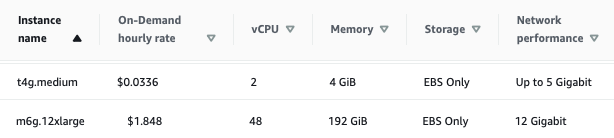
\includegraphics[width=\textwidth]{img/stats/hourly_cost.png}
\caption{The screenshot taken from the AWS pricing site shows that it is more cost effective to instantiate many nodes with 2 CPUs, rather than one large machine with many.}
\label{fig:cost}
\end{figure}

\FloatBarrier%



% % got instructions to build CentOS8 from 
% % https://hub.docker.com/_/centos?tab=description&page=1&ordering=last_updated
% % Docker file modified from 
% % https://github.com/CentOS/sig-cloud-instance-images/blob/ccd17799397027acf9ee6d660e75b8fce4c852e8/docker/Dockerfile 


% % SOURCE https://research.cs.wisc.edu/htcondor/manual/v8.6/3_16Setting_Up.html

% % no $HOME directory: condor user in wokder nnodes https://github.com/kubernetes/kubeadm/issues/2361.... 

\section{Applying Concepts from the BDP2 Course to the Non-Trivial Application}
The architecture described may be improved by implementing auto-scaling the number of worker nodes in the cluster.
Further, it would be possible to make use of Docker Hub and GitHub for configuring autobuilds of Docker images which allow automatized updating of an image when ever modifications are made to an existing container via a simple commit.
Additional modification could be done by using Docker Swarm or Kubernetes cluster, to orchestrate a multitude of containers.
Another possible solution is to use a serverless computing system like AWS Lambda or OpenFaaS (possibly on a self-scaling Kubernetes cluster).
The management of the latter requires however specialized knowledge and additional tools such as \texttt{kubectl CLI}, while it is more is more rich in functionality than Docker Swarm.

Considering the file system, it is worth noting that by configuring Docker to include a scratch directory in the host machine where the job is initiated, by bind mounting a volume permanently, we have tied the containers to the host. 
We could avoid this by using AWS S3 bucket, which allows to obtain unique links to buckets of files.
The S3 bucket has the advantage of employing a pay per use pricing model, as opposed to the EBS volumes where we pay for the entire capacity, regardless of space used.

% Zac, [20 Jun 2021 at 16:45:39]:
% Bottou, Léon, and Chih-Jen Lin. "Support vector machine solvers." Large scale kernel machines (2007): 301-320.

% https://www.researchgate.net/post/What-is-the-running-time-complexity-of-SVM-and-ANN
% AWS pricing:\\
% \texttt{https://aws.amazon.com/pricing}

% \section{References}
\printbibliography

\begin{figure}[!h]
\center
    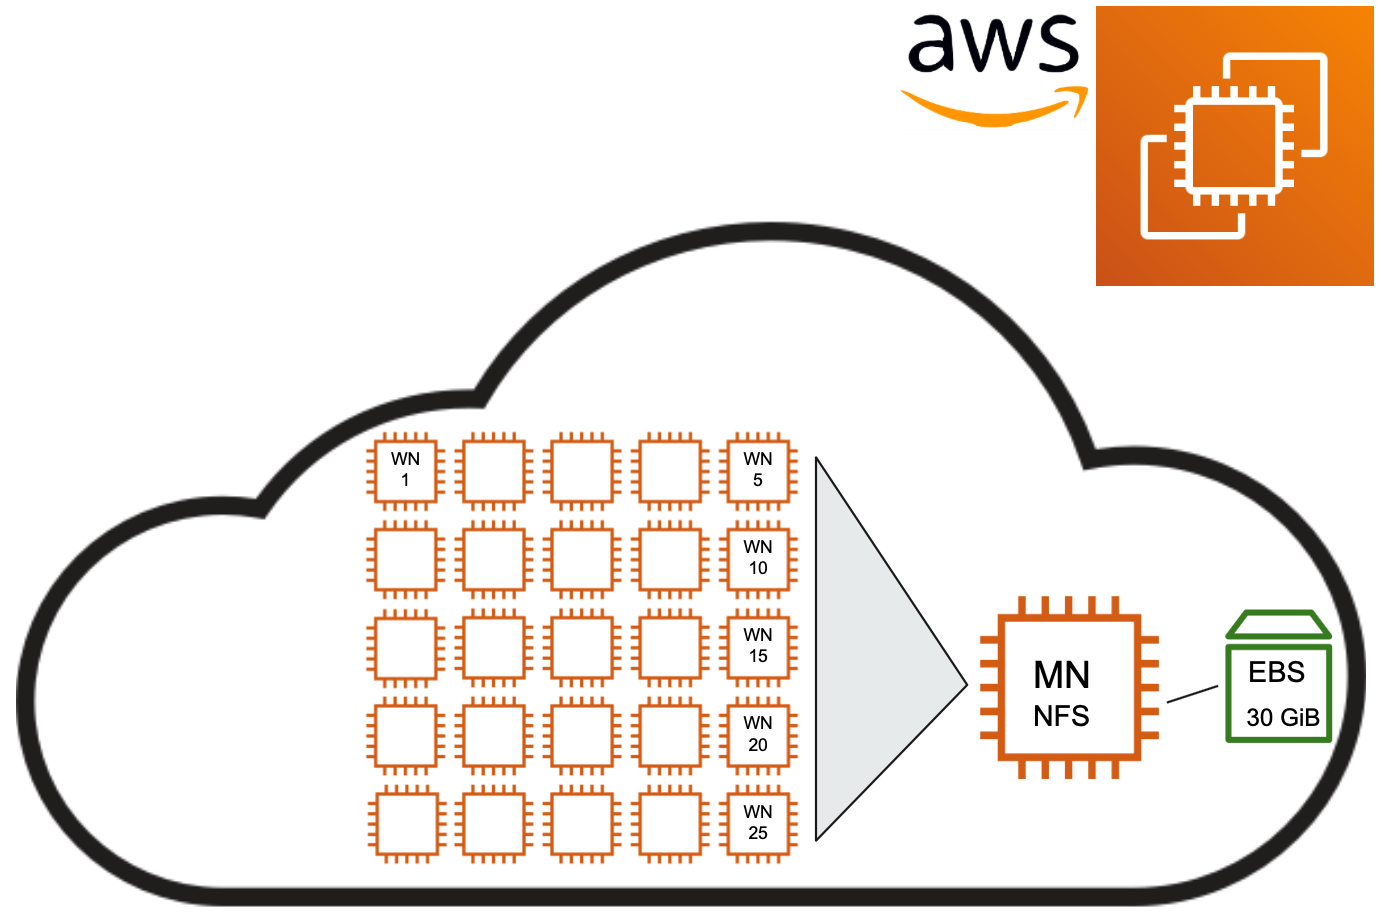
\includegraphics[width=0.7\textwidth]{img/usecase_iaas.png}
\caption{Proposed infrastructure of cluster: 25 worker nodes (WN) and 1 main node (MN) all of the type t4g.medium with 2 vCPU and 4 GiB of RAM. The main bottle neck of the infrastructure lies in the data transfer between main node and worker nodes and may lead to a higher run-time than the one proposed we modelled with the data available to us.}
\label{fig:infrastr}
\end{figure}

\begin{figure}[!h]
\center
    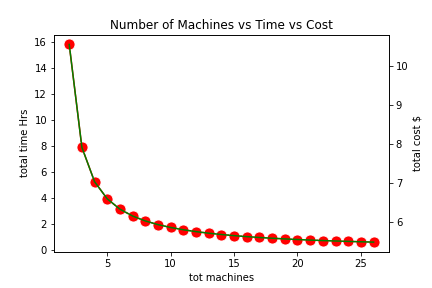
\includegraphics[width=0.6\textwidth]{img/n_machines_time_cost.png}
\caption{Note that the price and run-time remain roughly the same once the cluster reaches a size of 20 nodes.}
\label{fig:n_machines_vs_cost}
\end{figure}

\end{document}